% GNUPLOT: LaTeX picture with Postscript
\begingroup
  \makeatletter
  \providecommand\color[2][]{%
    \GenericError{(gnuplot) \space\space\space\@spaces}{%
      Package color not loaded in conjunction with
      terminal option `colourtext'%
    }{See the gnuplot documentation for explanation.%
    }{Either use 'blacktext' in gnuplot or load the package
      color.sty in LaTeX.}%
    \renewcommand\color[2][]{}%
  }%
  \providecommand\includegraphics[2][]{%
    \GenericError{(gnuplot) \space\space\space\@spaces}{%
      Package graphicx or graphics not loaded%
    }{See the gnuplot documentation for explanation.%
    }{The gnuplot epslatex terminal needs graphicx.sty or graphics.sty.}%
    \renewcommand\includegraphics[2][]{}%
  }%
  \providecommand\rotatebox[2]{#2}%
  \@ifundefined{ifGPcolor}{%
    \newif\ifGPcolor
    \GPcolorfalse
  }{}%
  \@ifundefined{ifGPblacktext}{%
    \newif\ifGPblacktext
    \GPblacktexttrue
  }{}%
  % define a \g@addto@macro without @ in the name:
  \let\gplgaddtomacro\g@addto@macro
  % define empty templates for all commands taking text:
  \gdef\gplbacktext{}%
  \gdef\gplfronttext{}%
  \makeatother
  \ifGPblacktext
    % no textcolor at all
    \def\colorrgb#1{}%
    \def\colorgray#1{}%
  \else
    % gray or color?
    \ifGPcolor
      \def\colorrgb#1{\color[rgb]{#1}}%
      \def\colorgray#1{\color[gray]{#1}}%
      \expandafter\def\csname LTw\endcsname{\color{white}}%
      \expandafter\def\csname LTb\endcsname{\color{black}}%
      \expandafter\def\csname LTa\endcsname{\color{black}}%
      \expandafter\def\csname LT0\endcsname{\color[rgb]{1,0,0}}%
      \expandafter\def\csname LT1\endcsname{\color[rgb]{0,1,0}}%
      \expandafter\def\csname LT2\endcsname{\color[rgb]{0,0,1}}%
      \expandafter\def\csname LT3\endcsname{\color[rgb]{1,0,1}}%
      \expandafter\def\csname LT4\endcsname{\color[rgb]{0,1,1}}%
      \expandafter\def\csname LT5\endcsname{\color[rgb]{1,1,0}}%
      \expandafter\def\csname LT6\endcsname{\color[rgb]{0,0,0}}%
      \expandafter\def\csname LT7\endcsname{\color[rgb]{1,0.3,0}}%
      \expandafter\def\csname LT8\endcsname{\color[rgb]{0.5,0.5,0.5}}%
    \else
      % gray
      \def\colorrgb#1{\color{black}}%
      \def\colorgray#1{\color[gray]{#1}}%
      \expandafter\def\csname LTw\endcsname{\color{white}}%
      \expandafter\def\csname LTb\endcsname{\color{black}}%
      \expandafter\def\csname LTa\endcsname{\color{black}}%
      \expandafter\def\csname LT0\endcsname{\color{black}}%
      \expandafter\def\csname LT1\endcsname{\color{black}}%
      \expandafter\def\csname LT2\endcsname{\color{black}}%
      \expandafter\def\csname LT3\endcsname{\color{black}}%
      \expandafter\def\csname LT4\endcsname{\color{black}}%
      \expandafter\def\csname LT5\endcsname{\color{black}}%
      \expandafter\def\csname LT6\endcsname{\color{black}}%
      \expandafter\def\csname LT7\endcsname{\color{black}}%
      \expandafter\def\csname LT8\endcsname{\color{black}}%
    \fi
  \fi
  \setlength{\unitlength}{0.0500bp}%
  \begin{picture}(8640.00,5040.00)%
    \gplgaddtomacro\gplbacktext{%
    }%
    \gplgaddtomacro\gplfronttext{%
      \csname LTb\endcsname%
      \put(0,-124){\makebox(0,0){\centering\scriptsize$\mathsf{1}$}}%
      \put(1440,-124){\makebox(0,0){\centering\scriptsize\textsf{Gain}}}%
      \put(2879,-124){\makebox(0,0){\centering\scriptsize$\mathsf{0.000}$}}%
      \put(4319,-124){\makebox(0,0){\centering\scriptsize\textsf{Unused}}}%
      \put(5759,-124){\makebox(0,0){\centering\scriptsize$\mathsf{0.000}$}}%
      \put(7198,-124){\makebox(0,0){\centering\scriptsize$\mathsf{0.000}$}}%
      \put(8638,-124){\makebox(0,0){\centering\scriptsize$\mathsf{1.000}$}}%
      \put(4473,458){\makebox(0,0){\centering\scriptsize $\mathsf{\phantom{0\;00}0.000}$}}%
      \put(0,5165){\makebox(0,0){\centering\scriptsize$\mathsf{418}$}}%
      \put(1440,5165){\makebox(0,0){\centering\scriptsize\textsf{Gain ratio}}}%
      \put(2879,5165){\makebox(0,0){\centering\scriptsize$\mathsf{100.000}$}}%
      \put(4319,5165){\makebox(0,0){\centering\scriptsize$\mathsf{100.000}$}}%
      \put(5759,5165){\makebox(0,0){\centering\scriptsize$\mathsf{10\;000.000}$}}%
      \put(7198,5165){\makebox(0,0){\centering\scriptsize$\mathsf{75.000}$}}%
      \put(8638,5165){\makebox(0,0){\centering\scriptsize$\mathsf{31.833}$}}%
      \put(0,5659){\makebox(0,0){\centering\small\textsf{\phantom{p}Minimum\phantom{p}}}}%
      \put(0,5442){\makebox(0,0){\centering\small\textsf{\phantom{p}examples\phantom{p}}}}%
      \put(1440,5659){\makebox(0,0){\centering\small\textsf{\phantom{p}Test\phantom{p}}}}%
      \put(1440,5442){\makebox(0,0){\centering\small\textsf{\phantom{p}heuristic\phantom{p}}}}%
      \put(2879,5659){\makebox(0,0){\centering\small\textsf{\phantom{p}Pessimistic\phantom{p}}}}%
      \put(2879,5442){\makebox(0,0){\centering\small\textsf{\phantom{p}confidence\phantom{p}}}}%
      \put(4319,5659){\makebox(0,0){\centering\small\textsf{\phantom{p}Fisher's\phantom{p}}}}%
      \put(4319,5442){\makebox(0,0){\centering\small\textsf{\phantom{p}confidence\phantom{p}}}}%
      \put(5759,5659){\makebox(0,0){\centering\small\textsf{\phantom{p}Attribute\phantom{p}}}}%
      \put(5759,5442){\makebox(0,0){\centering\small\textsf{\phantom{p}redundancy\phantom{p}}}}%
      \put(7198,5442){\makebox(0,0){\centering\small\textsf{\phantom{p}}${\cal E}_{G}$\textsf{\phantom{p}}}}%
      \put(8638,5442){\makebox(0,0){\centering\small\textsf{\phantom{p}}${\cal E}_{C}$\textsf{\phantom{p}}}}%
      \put(-355,1112){\makebox(0,0){\scriptsize $\mathsf{\phantom{0\;0000.}93}$}}%
      \put(2522,2154){\makebox(0,0){\scriptsize $\mathsf{\phantom{0\;0}43.945}$}}%
      \put(5402,1060){\makebox(0,0){\scriptsize $\mathsf{1\;972.656}$}}%
      \put(6841,1707){\makebox(0,0){\scriptsize $\mathsf{\phantom{0\;0}24.286}$}}%
      \put(8281,282){\makebox(0,0){\scriptsize $\mathsf{\phantom{0\;00}3.000}$}}%
    }%
    \gplbacktext
    \put(0,0){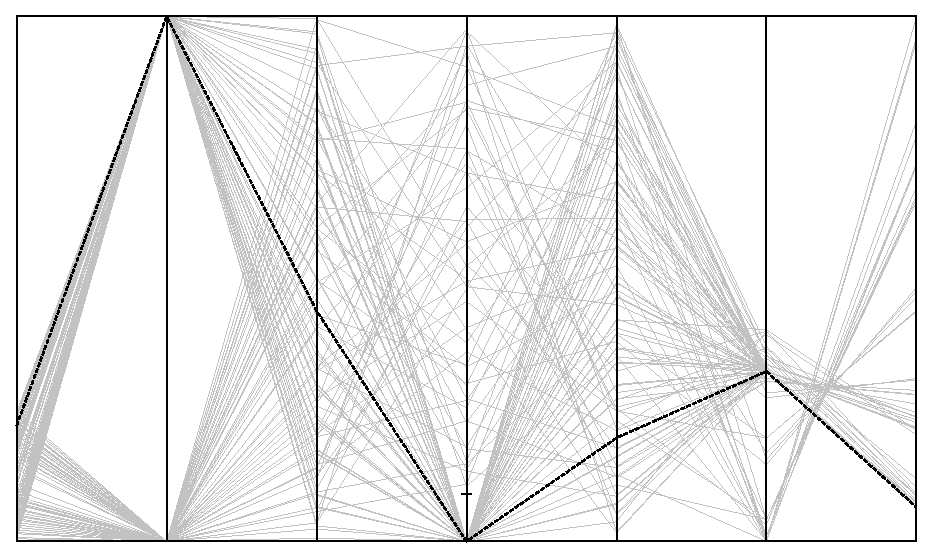
\includegraphics{c4-5_monks1_gnuplot_generalization}}%
    \gplfronttext
  \end{picture}%
\endgroup
